\PassOptionsToPackage{unicode=true}{hyperref} % options for packages loaded elsewhere
\PassOptionsToPackage{hyphens}{url}
%
\documentclass[]{article}
\usepackage{lmodern}
\usepackage{amssymb,amsmath}
\usepackage{ifxetex,ifluatex}
\usepackage{fixltx2e} % provides \textsubscript
\ifnum 0\ifxetex 1\fi\ifluatex 1\fi=0 % if pdftex
  \usepackage[T1]{fontenc}
  \usepackage[utf8]{inputenc}
  \usepackage{textcomp} % provides euro and other symbols
\else % if luatex or xelatex
  \usepackage{unicode-math}
  \defaultfontfeatures{Ligatures=TeX,Scale=MatchLowercase}
\fi
% use upquote if available, for straight quotes in verbatim environments
\IfFileExists{upquote.sty}{\usepackage{upquote}}{}
% use microtype if available
\IfFileExists{microtype.sty}{%
\usepackage[]{microtype}
\UseMicrotypeSet[protrusion]{basicmath} % disable protrusion for tt fonts
}{}
\IfFileExists{parskip.sty}{%
\usepackage{parskip}
}{% else
\setlength{\parindent}{0pt}
\setlength{\parskip}{6pt plus 2pt minus 1pt}
}
\usepackage{hyperref}
\hypersetup{
            pdfborder={0 0 0},
            breaklinks=true}
\urlstyle{same}  % don't use monospace font for urls
\usepackage{graphicx,grffile}
\makeatletter
\def\maxwidth{\ifdim\Gin@nat@width>\linewidth\linewidth\else\Gin@nat@width\fi}
\def\maxheight{\ifdim\Gin@nat@height>\textheight\textheight\else\Gin@nat@height\fi}
\makeatother
% Scale images if necessary, so that they will not overflow the page
% margins by default, and it is still possible to overwrite the defaults
% using explicit options in \includegraphics[width, height, ...]{}
\setkeys{Gin}{width=\maxwidth,height=\maxheight,keepaspectratio}
\setlength{\emergencystretch}{3em}  % prevent overfull lines
\providecommand{\tightlist}{%
  \setlength{\itemsep}{0pt}\setlength{\parskip}{0pt}}
\setcounter{secnumdepth}{0}
% Redefines (sub)paragraphs to behave more like sections
\ifx\paragraph\undefined\else
\let\oldparagraph\paragraph
\renewcommand{\paragraph}[1]{\oldparagraph{#1}\mbox{}}
\fi
\ifx\subparagraph\undefined\else
\let\oldsubparagraph\subparagraph
\renewcommand{\subparagraph}[1]{\oldsubparagraph{#1}\mbox{}}
\fi

% set default figure placement to htbp
\makeatletter
\def\fps@figure{htbp}
\makeatother


\date{}

\begin{document}

\hypertarget{header-n0}{%
\section{数据收集}\label{header-n0}}

数据来源:

\href{https://robo.datayes.com/v2/home}{萝卜投研}

用到的指标/变量:

\begin{enumerate}
\def\labelenumi{\arabic{enumi}.}
\item
  GDP(当季值)
\item
  沪深300收盘价(日度)
\item
  \href{https://baike.baidu.com/item/\%E7\%BB\%8F\%E6\%B5\%8E\%E6\%99\%AF\%E6\%B0\%94\%E6\%8C\%87\%E6\%95\%B0/6782162}{宏观经济景气指数}(先行值)
\item
  \href{https://baike.baidu.com/item/\%E7\%BB\%8F\%E6\%B5\%8E\%E6\%99\%AF\%E6\%B0\%94\%E6\%8C\%87\%E6\%95\%B0/6782162}{宏观经济景气指数}(一致值)
\end{enumerate}

\begin{quote}
一致指数是反映当前经济的基本走势,由工业生产、就业、\href{https://baike.baidu.com/item/\%E7\%A4\%BE\%E4\%BC\%9A\%E9\%9C\%80\%E6\%B1\%82}{社会需求}(投资、消费、外贸)、社会收入(国家税收、企业利润、\href{https://baike.baidu.com/item/\%E5\%B1\%85\%E6\%B0\%91\%E6\%94\%B6\%E5\%85\%A5}{居民收入})等4个方面合成;先行指数是由一组领先于一致指数的\href{https://baike.baidu.com/item/\%E5\%85\%88\%E8\%A1\%8C\%E6\%8C\%87\%E6\%A0\%87}{先行指标}合成,用于对经济未来的走势进行预测
\end{quote}

\begin{enumerate}
\def\labelenumi{\arabic{enumi}.}
\item
  活期存款利率(月度)
\item
  CPI(当月同比)
\item
  货币供应量M2(同比)
\item
  定期存款利率(1年整存整取)
\item
  \href{https://baike.baidu.com/item/\%E5\%9B\%BD\%E6\%88\%BF\%E6\%99\%AF\%E6\%B0\%94\%E6\%8C\%87\%E6\%95\%B0/7035576}{国房景气指数}
\end{enumerate}

\begin{quote}
全国房地产开发景气指数(简称``国房景气指数'')遵循经济周期波动的理论,以景气循环理论与景气循环分析方法为依据,运用时间序列、多元统计、计量经济分析方法,以房地产开发投资为基准指标

国房景气指数100点是最合适的景气水平,95至105点之间为适度景气水平,95以下为较低景气水平,105以上为偏高景气水平
\end{quote}

\hypertarget{header-n30}{%
\section{数据处理}\label{header-n30}}

\hypertarget{header-n31}{%
\subsection{数据频率转化}\label{header-n31}}

\hypertarget{header-n32}{%
\subsubsection{GDP}\label{header-n32}}

\begin{enumerate}
\def\labelenumi{\arabic{enumi}.}
\item
  首先,GDP的季度值存在季节趋势

  \begin{figure}
  \centering
  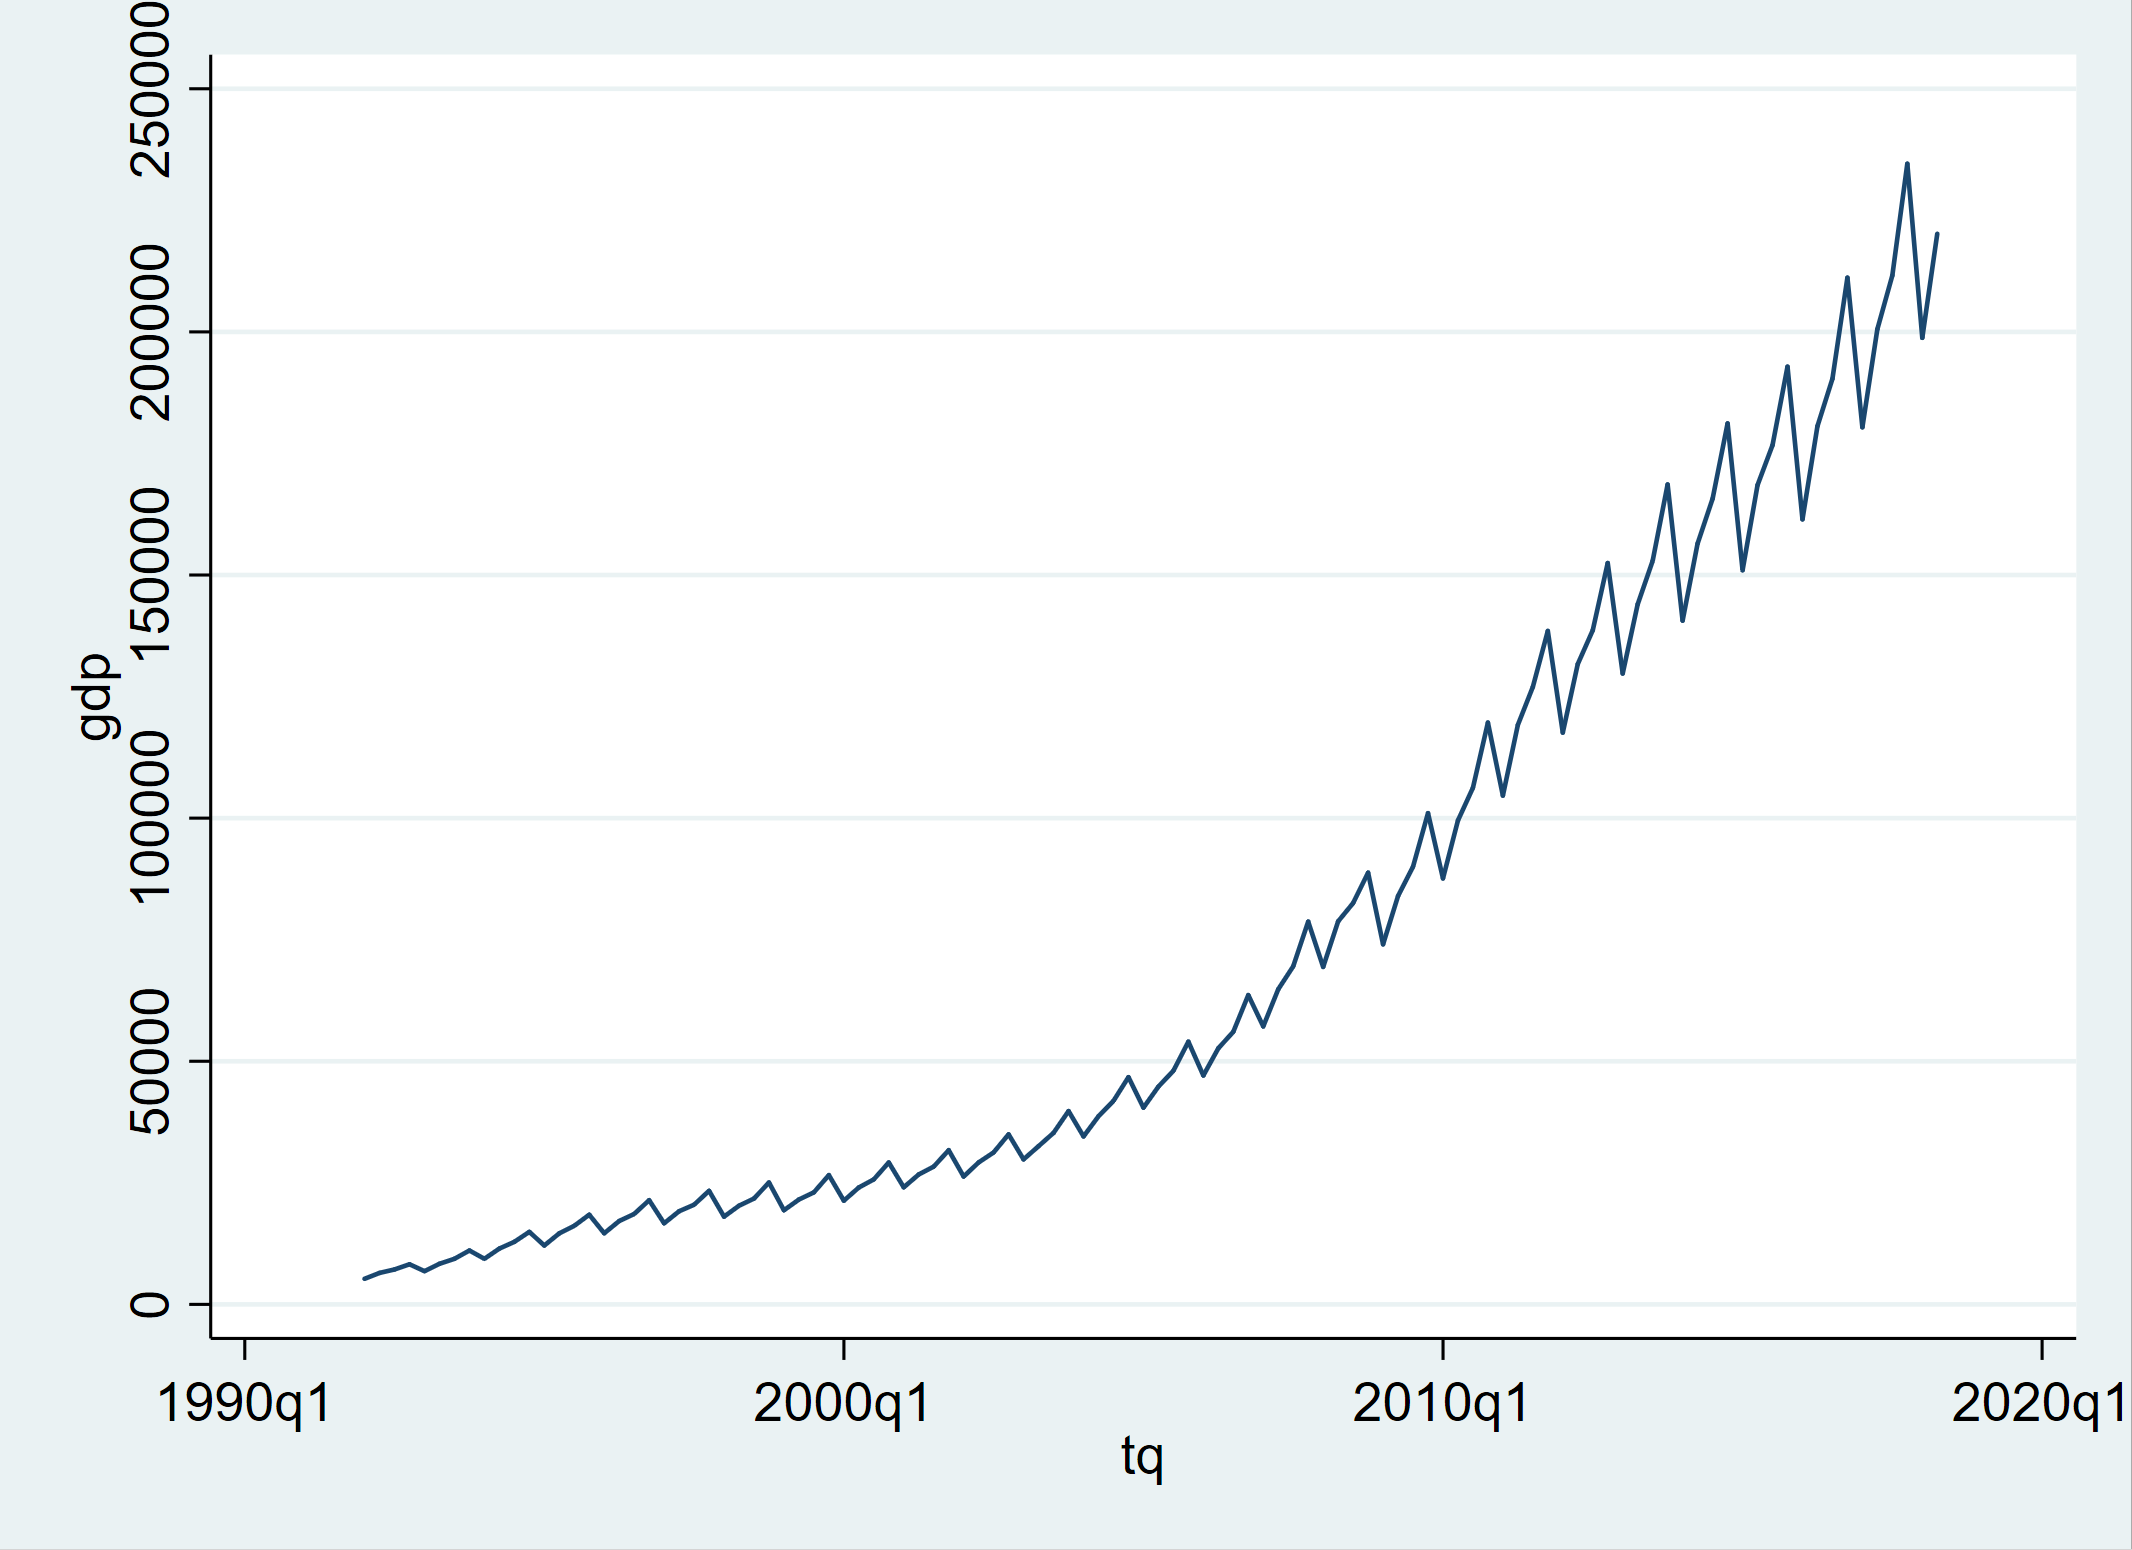
\includegraphics{D:/OneDrive - stu.xjtu.edu.cn/SurfaceStudy/科研训练/GDP季节趋势.png}
  \caption{}
  \end{figure}

  为了消除这种季节趋势,我们需要对GDP季度值数据进行\textbf{季节调整}

  \hypertarget{header-n38}{%
  \paragraph{季节调整}\label{header-n38}}

  季节调整通常通过估计\textbf{``季节因子(seasonal
  factor)''}来进行。根据季节因子起作用的方法,主要分为\textbf{``加法季节因子(additive
  seasonal factor)''},与\textbf{``乘法季节因子(multiplicative seasonal
  factor)''}。

  加法因子意味着对所有的第一月(或第一季)加上相同的季节因子,以此类推。

  \[Y_t=TC_t+S_t+I_t\\
  其中\\
  Y_t为原序列\\TC_t为趋势循环要素\\T反映的是经济现象的长期演变方向\\C是时间序列表现出的持续的周期性波动\\由于测算趋势在实际工作中有一定的难度,因此一般把趋势与循环放在一起不再进行区分\\S_t为季节要素,反应不同年份相同季节的周期性变化\\而I_t为不规则要素,如罢工、自然灾害对经济活动的影响\]

  乘法模型的数学表达式如下:

  \[Y_t=TC_t\times S_t\times I_t\\
  或者以对数形式\\
  ln{Y_t}=ln{TC_t}+ln{S_t}+ln{I_t}\]

  \begin{center}\rule{0.5\linewidth}{\linethickness}\end{center}

  以上为季节调整的主要两种模型。

  一般来说如果4种成分是相互独立的就用加法模型,若相互有关联就用乘法模型。

  季节调整的具体方法有多种,不同方法有不一样的结果,所以这是一项有主观性的工作。目前来说最权威的方法是美国普查局设计的专门用于计算机上运行的\textbf{X12}方法,而在这里我们使用\textbf{移动平均法}进行季节调整。

  \hypertarget{header-n48}{%
  \subparagraph{移动平均法}\label{header-n48}}

  对于季度数据,我们进行4项移动平均。假设此时我们要求t=3时点上的4项平均:

  \[MA_{2.5}=\frac{y_1+y_2+y_3+y_4}4\\
  MA_{3.5}=\frac{y_2+y_3+y_4+y_5}4\\\]

  定义相应的中心化移动平均值为:

  \[MA_3=\frac{1}{2}(MA_{2.5}+MA_{3.5})\]

  以此类推,中心化移动平均的一般公式为:

  \[MA_t=\frac{1}2(\frac{y_{t-2}+y_{t-1}+y_{t}+y_{t+1}}{4}+\frac{+y_{t-1}+y_{t}+y_{t+1}+{y_{t+2}}}{4})\\
  =\frac{1}{4}(\frac{y_{t-2}}{2}+y_{t-1}+y_t+y_{t+1}+\frac{y_{t+2}}{2})\]

  移动平均法季节调整的步骤为

  \begin{enumerate}
  \def\labelenumii{\arabic{enumii}.}
  \item
    对季度数据进行4项中心化移动平均,得到趋势循环序列TC
  \item
    计算季节要素和不规则要素之和

    \[SI_t=S_t+I_t=Y_t-TC_t\]
  \item
    对于季度数据

    \[SI_t\]

    分别计算其对应的平均值,如求第二季度的平均值,则求整个数据期间所有第二季度的数据的平均值
  \item
    调整季节因子,使它们的和为0:

    \[S_t\equiv s_t-\frac{1}k\sum_{j=1}^{k}s_j\]

    其中k=4
  \item
    计算季节调整的最终结果:

    \[TCI_t\equiv Y_t-S_t\]
  \end{enumerate}
\end{enumerate}

\begin{verbatim}
  经过季节调整以后的数据:

  ![1535609576350](D:\OneDrive - stu.xjtu.edu.cn\SurfaceStudy\科研训练\1535609576350.png)

  同时对比一下x12调整方法与移动平均法得到的GDP序列:

  ![1535609834831](D:\OneDrive - stu.xjtu.edu.cn\SurfaceStudy\科研训练\1535609834831.png)

  可见GDP作为十分稳当的季度数据在不同的季节调整方法下差异很小
\end{verbatim}

\begin{enumerate}
\def\labelenumi{\arabic{enumi}.}
\item
  GDP是最重要的变量,但是我国GDP统计为一个季度一次,因此需要将GDP转化为\textbf{月度频率数据},这是数据\textbf{频率由低到高}的转化,存在一些不可避的问题。如果我们学过\textbf{随机过程}那么可以用\textbf{MIDAS模型},这也是目前最热门的方法。因为知识受限,我们采用二次匹配方法直接转化数据频率的方法,针对低频的序列拟合局部二次多项式,然后使用该多项式填充相关的高频序列的所有观测值。
\end{enumerate}

经过频率转化以后的gdp走势图如下(这里截取了从2002年开始到现在的观测值):

\begin{figure}
\centering
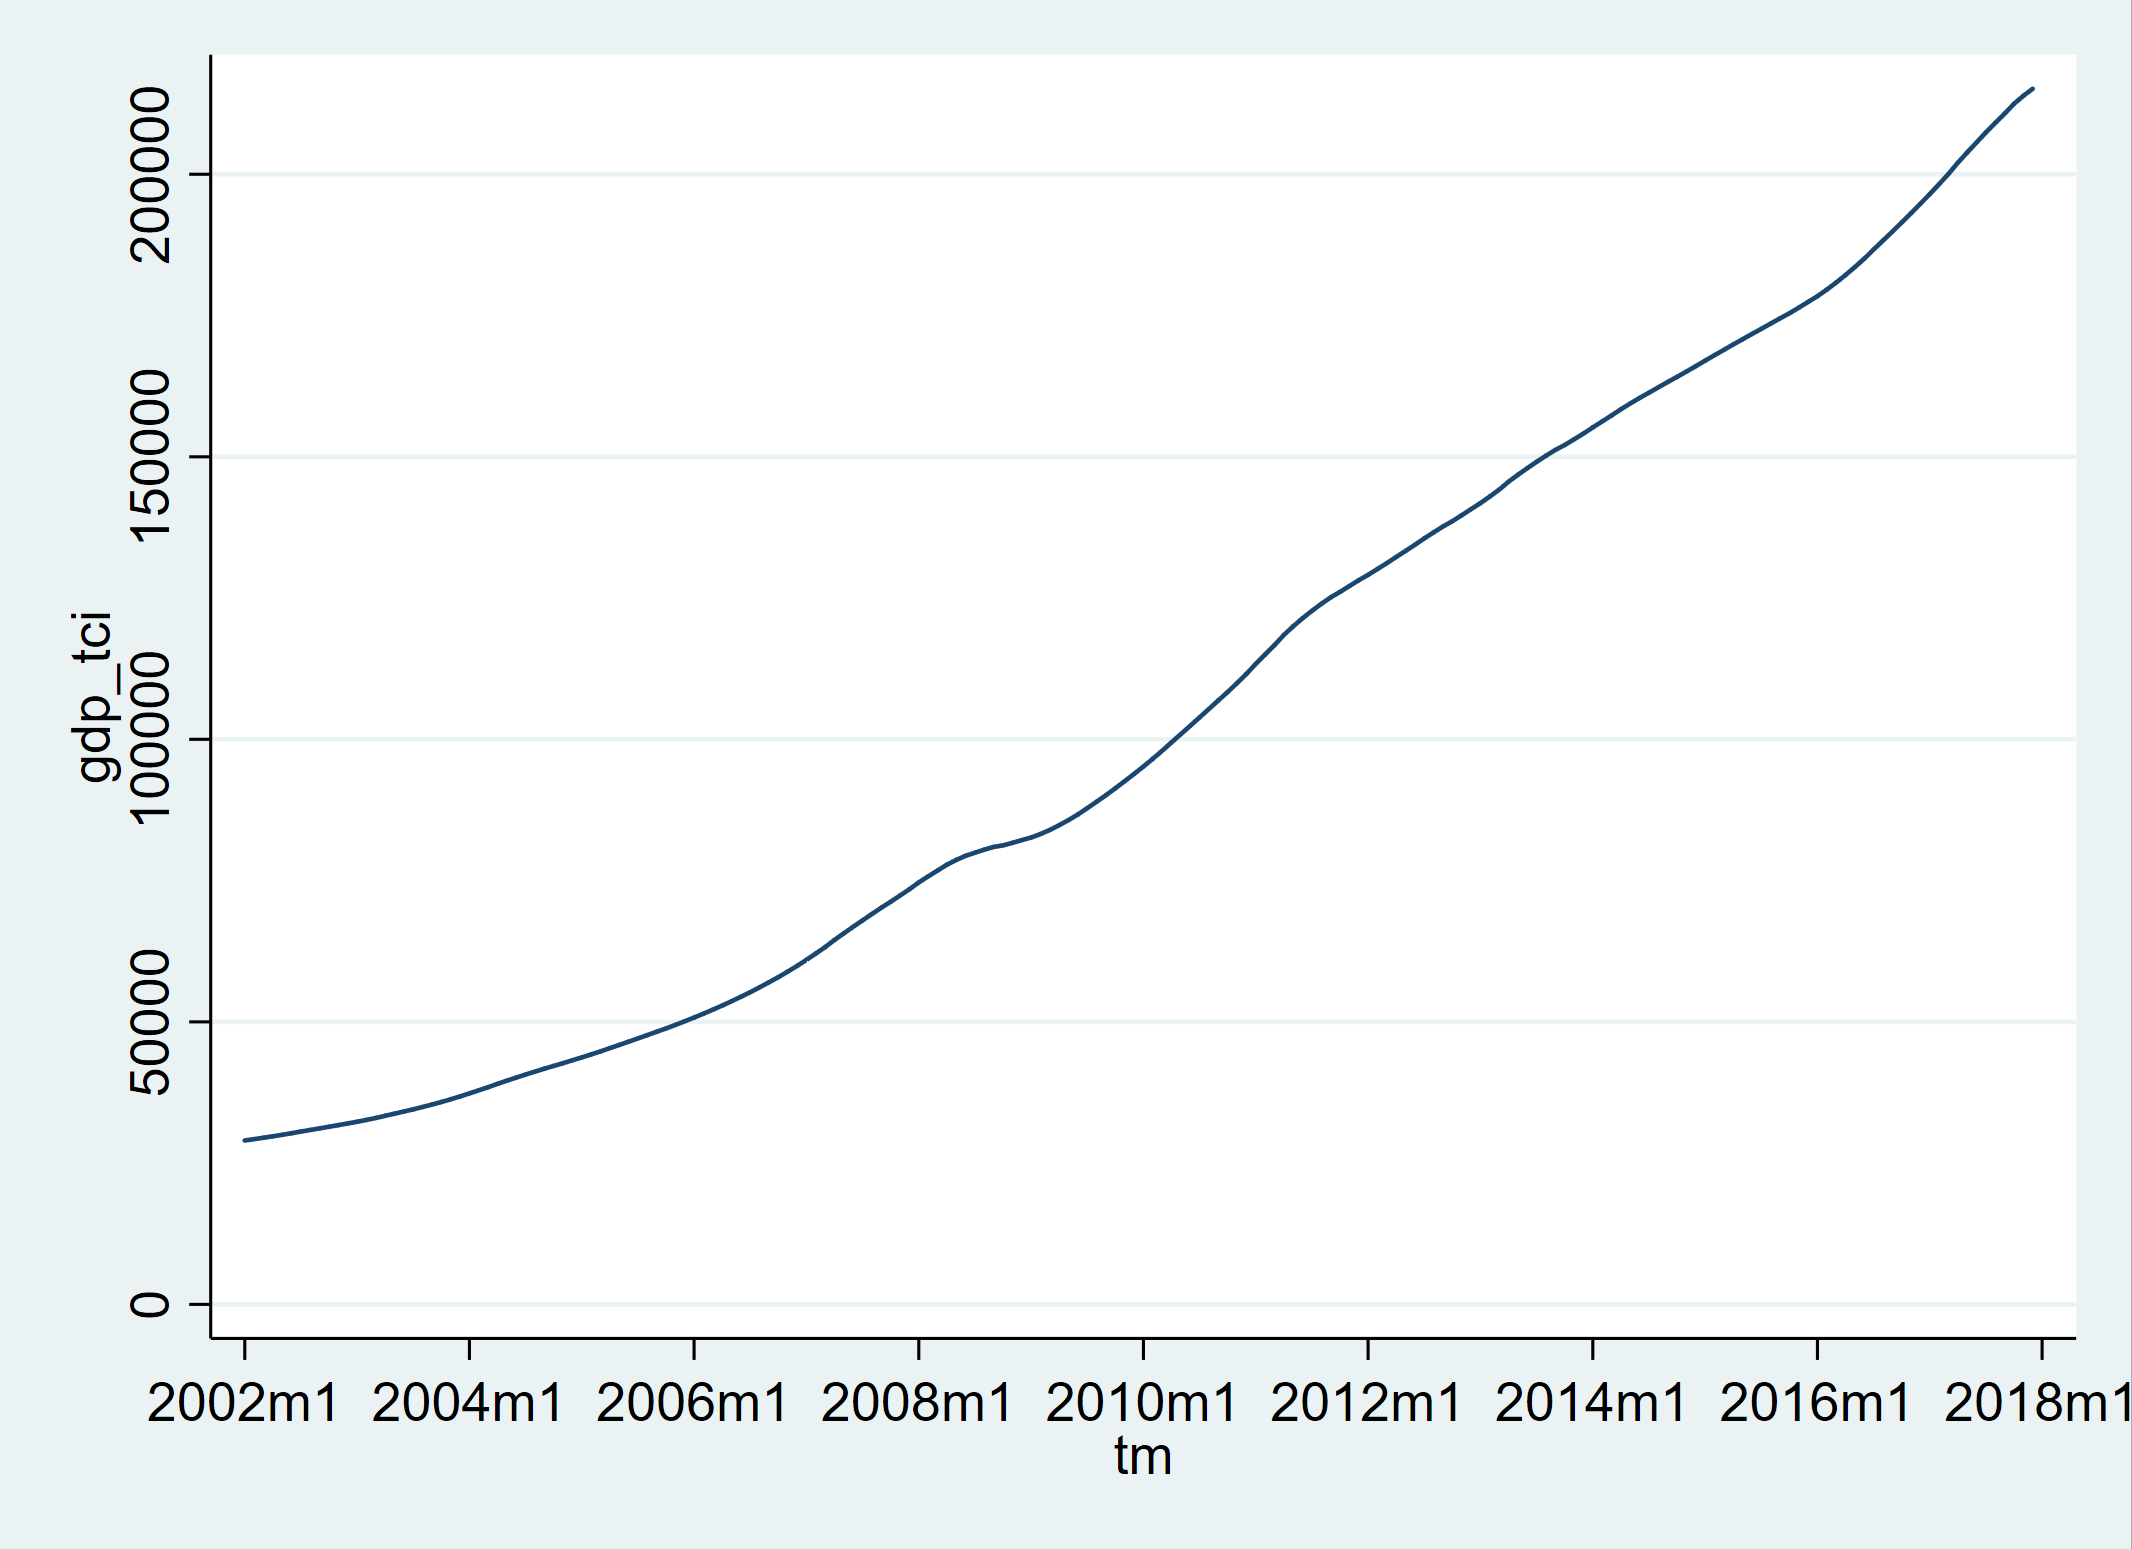
\includegraphics{D:/OneDrive - stu.xjtu.edu.cn/SurfaceStudy/科研训练/1535611948342.png}
\caption{}
\end{figure}

\hypertarget{header-n81}{%
\subsubsection{沪深300收盘价}\label{header-n81}}

沪深300收盘价是日度数据,每周一到周五(工作日)有观测值。我们将沪深300收盘价进行数据频率转化,转化为月度数据,这次是高频数据转低频。这里我们直接选取一个月内的平均值作为月度值。

频率转化前的HS300收盘价:

\begin{figure}
\centering
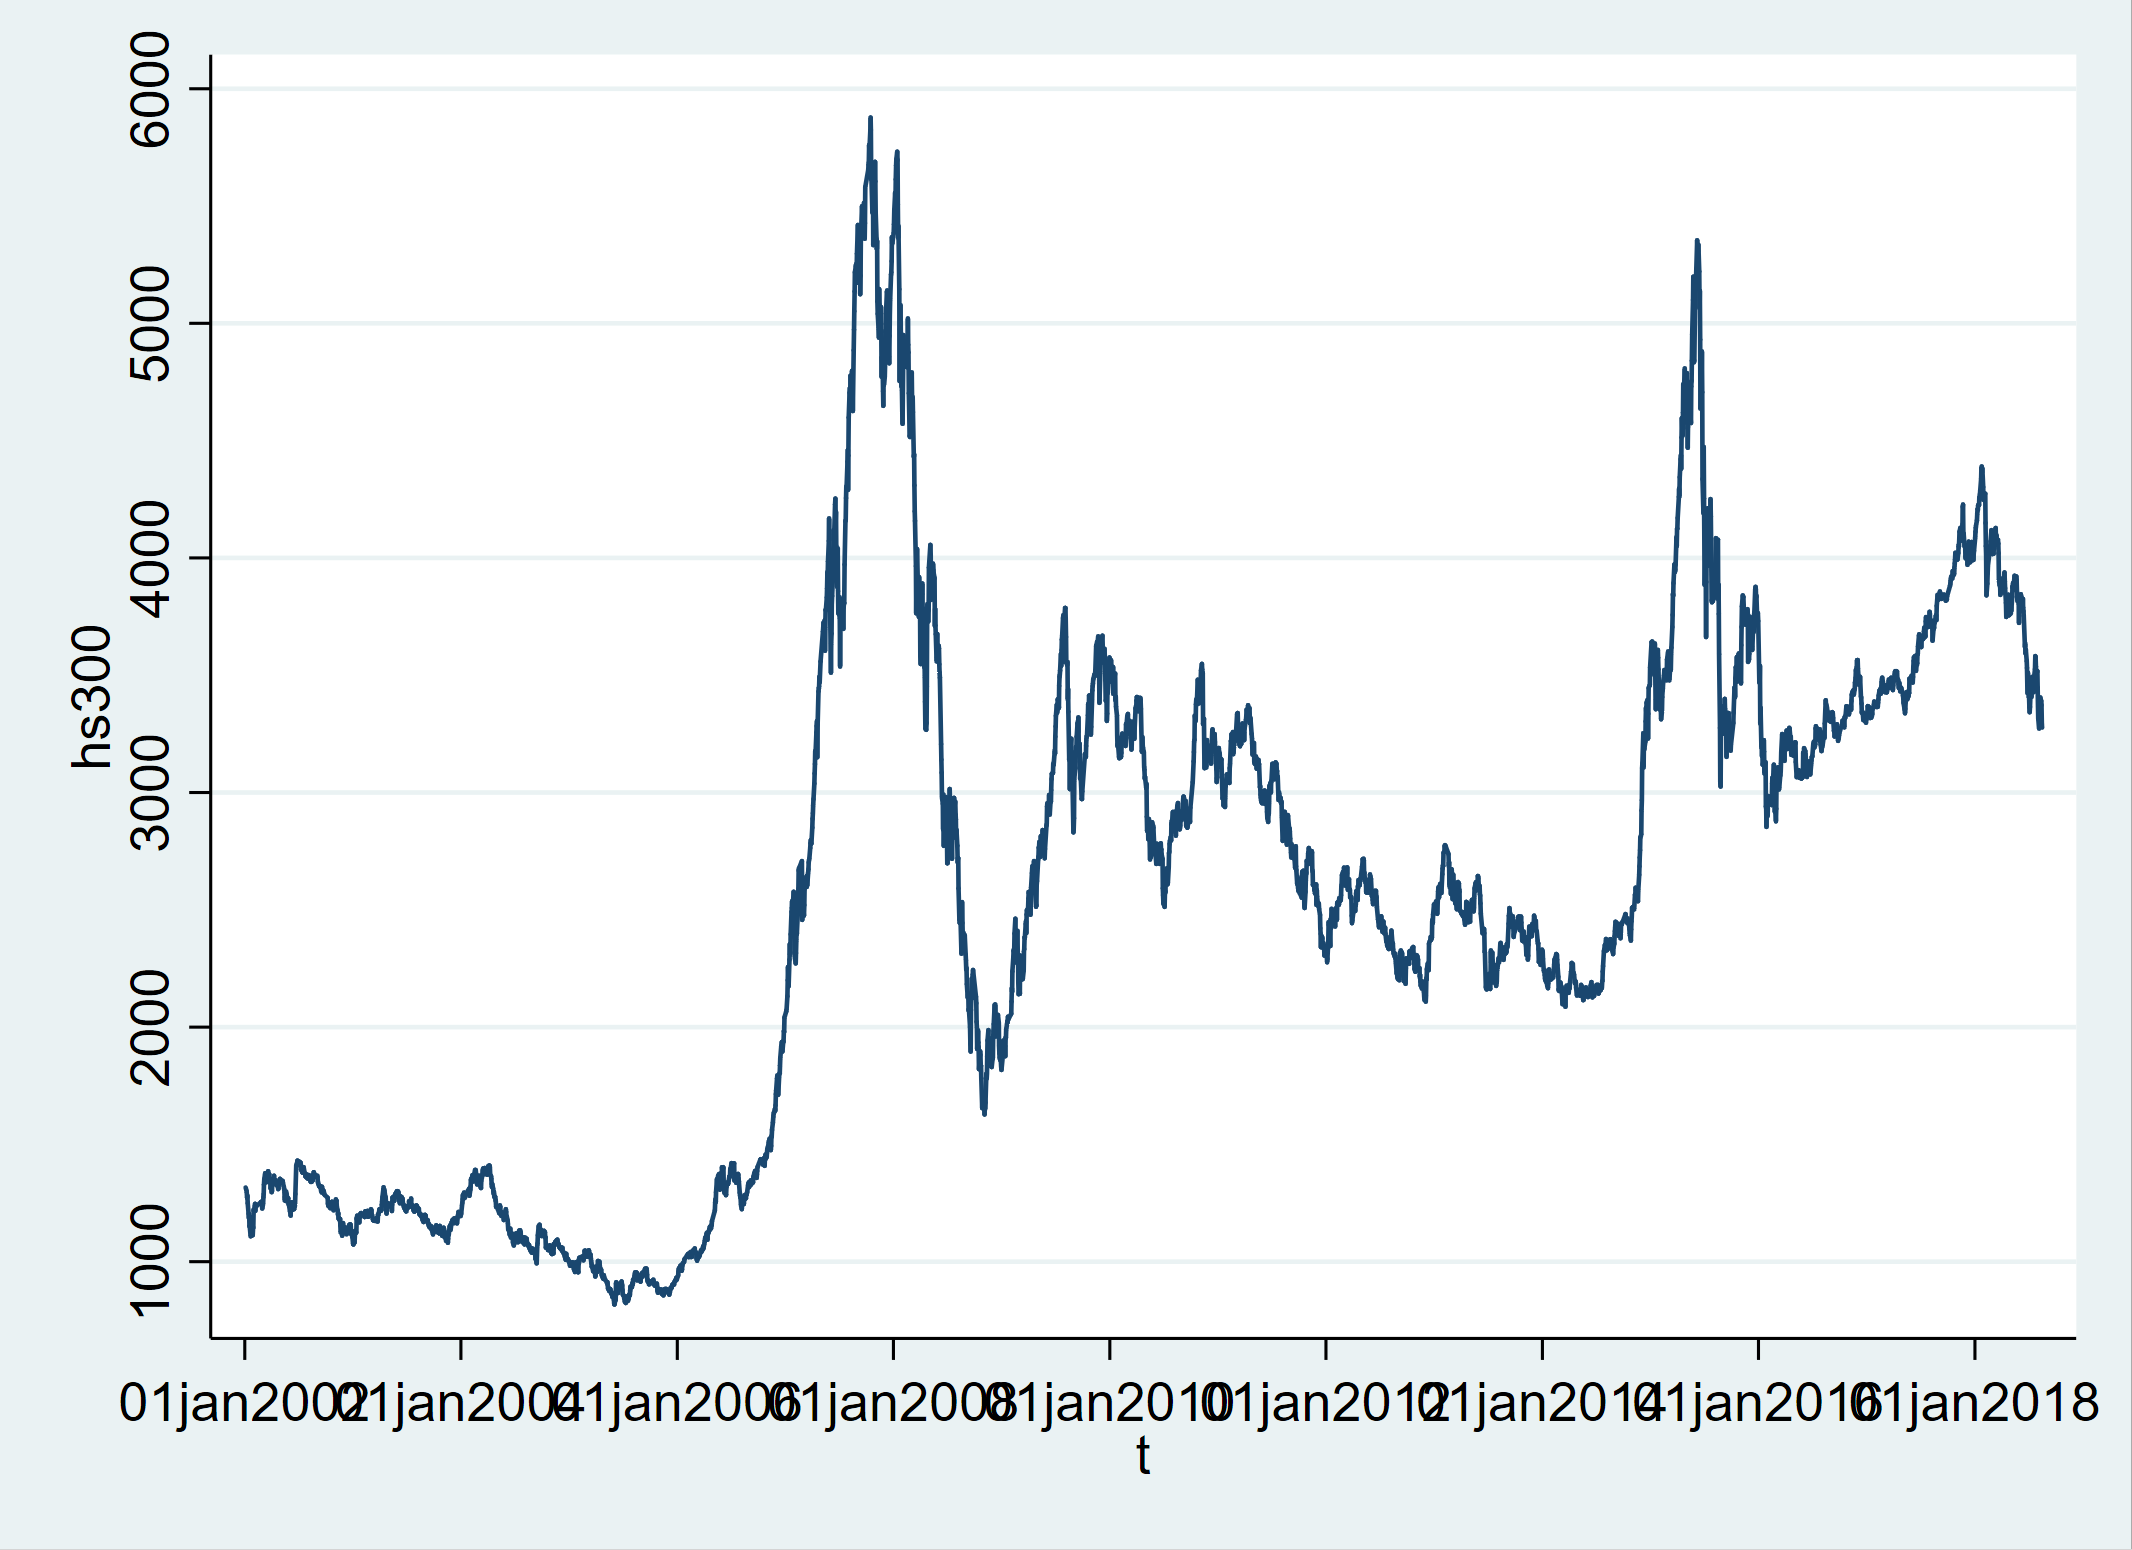
\includegraphics{D:/OneDrive - stu.xjtu.edu.cn/SurfaceStudy/科研训练/HS300.png}
\caption{}
\end{figure}

频率转化过后的HS300收盘价:

\begin{figure}
\centering
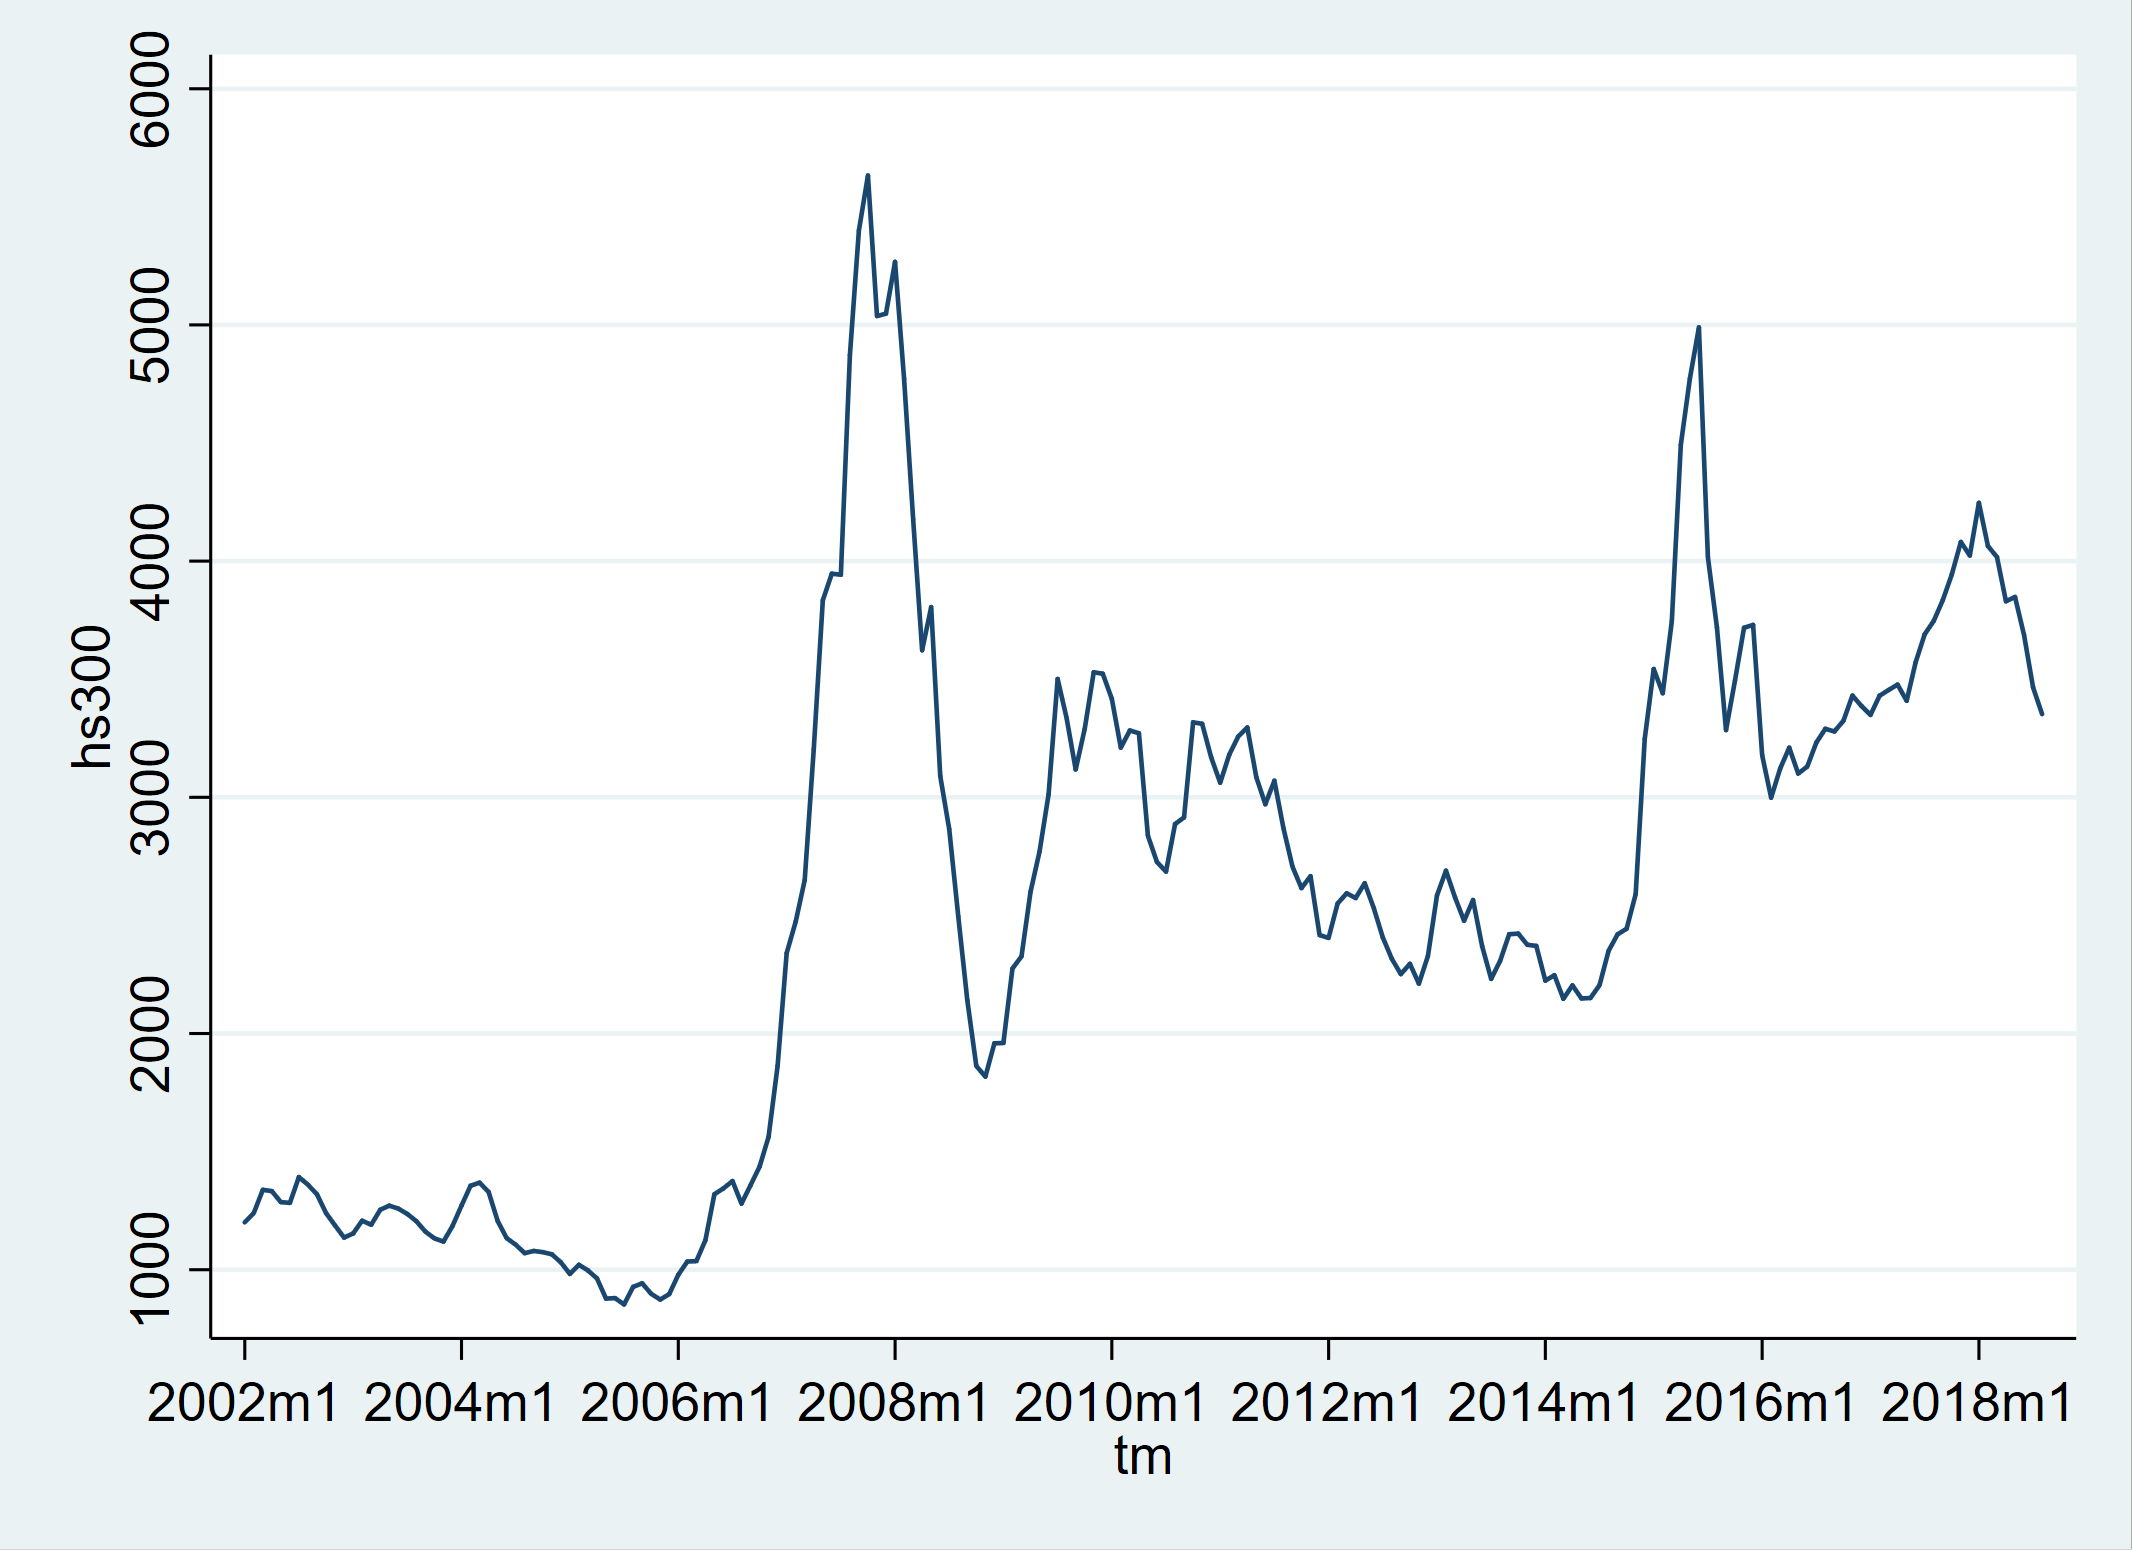
\includegraphics{D:/OneDrive - stu.xjtu.edu.cn/SurfaceStudy/科研训练/hs300频率转化绘图.png}
\caption{}
\end{figure}

\hypertarget{header-n89}{%
\subsubsection{数据整合}\label{header-n89}}

我们在处理GDP和HS300时候是在一个只有时间变量和GDP/HS300的dta文件下操作,同时我们还有其他频率已经是monthly的指标,所以我们要将他们合并到同一个dta中。这里用到stata的merge命令

\begin{verbatim}
merge 1:1 tm using gdp.dta , assert(1)
merge 1:1 tm using hs300.dta , assert(1)
\end{verbatim}

最后的dta文件见群文件

\hypertarget{header-n93}{%
\section{模型建立}\label{header-n93}}

首先我们检查变量的稳定性,发现所有的变量均不稳定且一阶单整

因此我们对变量做一阶差分以后建立向量自回归模型

\begin{figure}
\centering
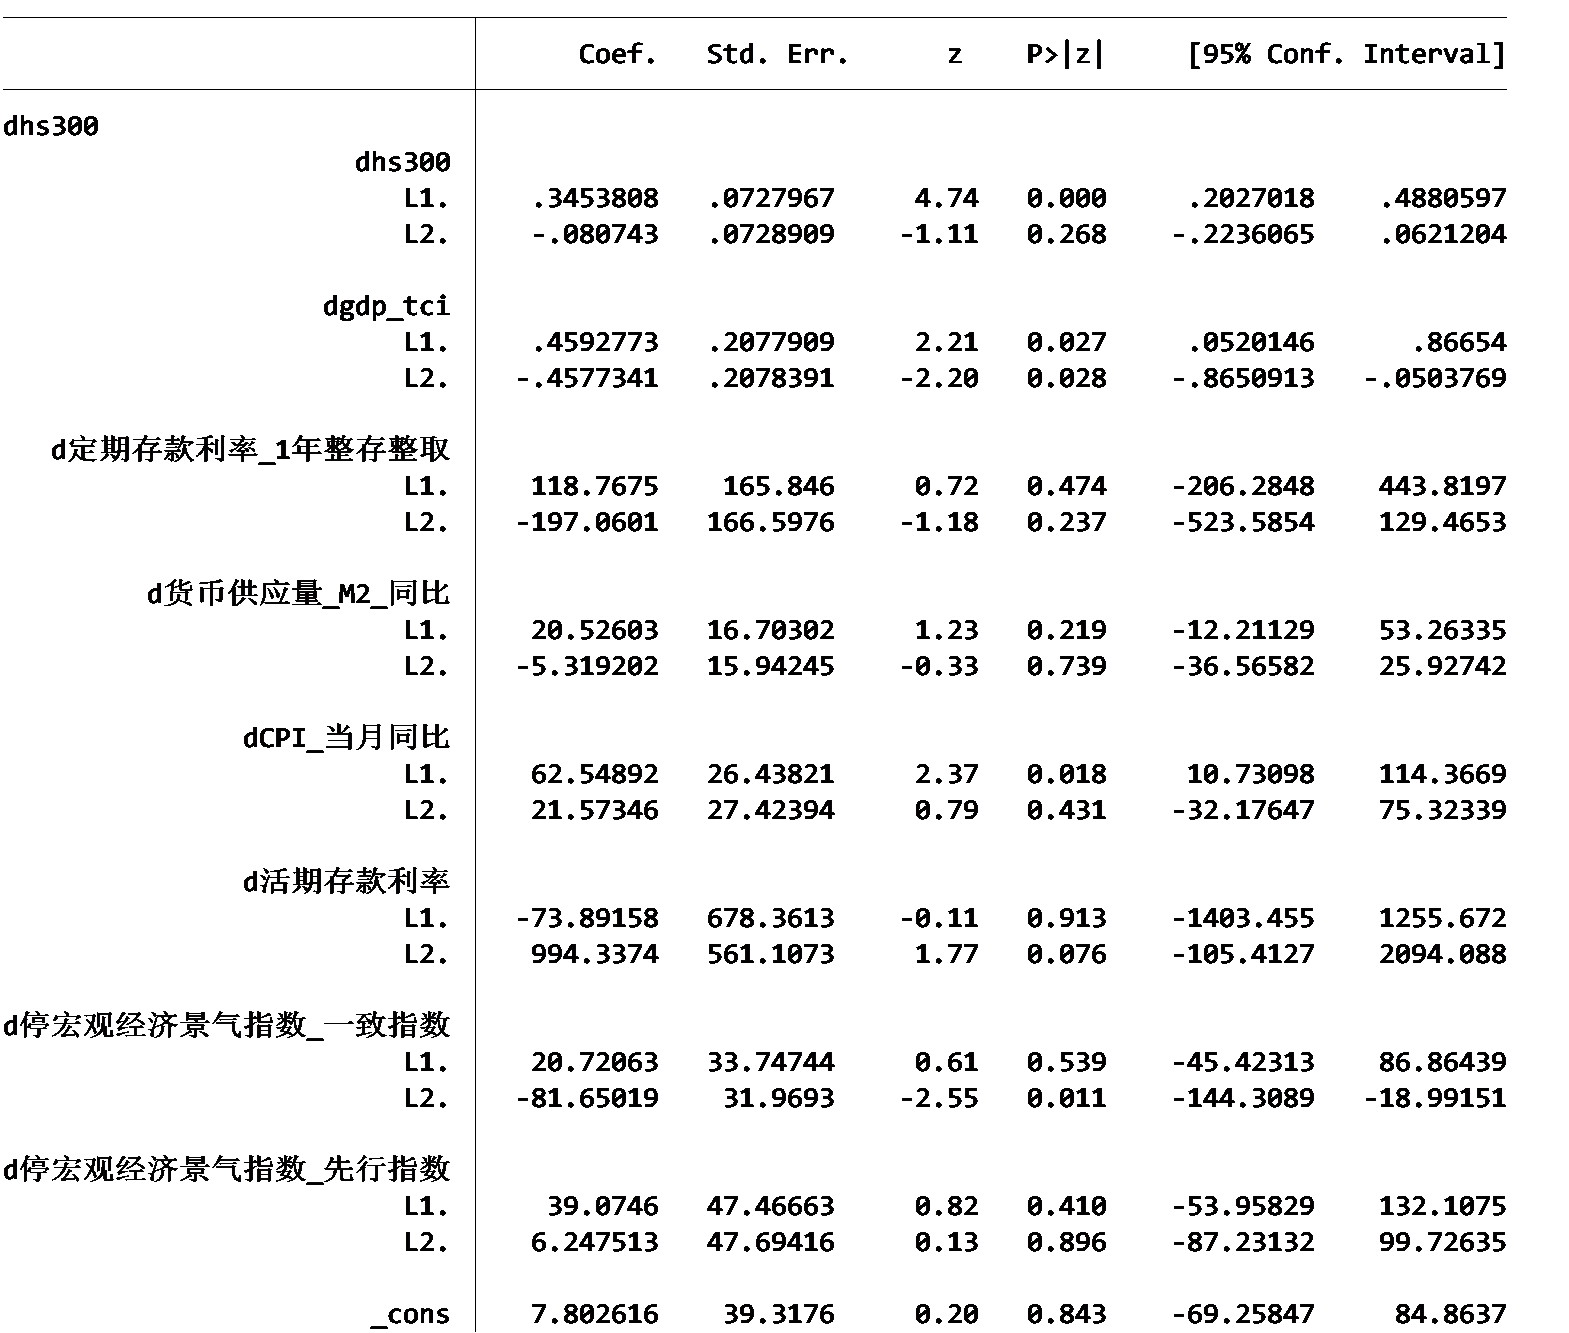
\includegraphics{D:/OneDrive - stu.xjtu.edu.cn/SurfaceStudy/科研训练/d var.png}
\caption{}
\end{figure}

对该模型做稳定性检验,发现该var模型是稳定的

\begin{figure}
\centering

\includegraphics{D:/OneDrive - stu.xjtu.edu.cn/SurfaceStudy/科研训练/varstable.png}
\caption{}
\end{figure}

\end{document}
